\section{Results}
\label{sec:results}

Table~\ref{tab:main} gives the main numbers and Figure~\ref{fig:budget} the budget curves. We first read off the
budget study, then the comparison between the learned policies and the search, then the ladder that attributes the
gain, then seeds, ablations and failure analysis.

\begin{table}[t]
  \centering\small
  \caption{Mean IoU after trim over the \nAttempted{} attempted cases (failed builds scored 0) at each piece budget,
  with the split at the 200-piece cap, validity and model-stability counts out of 53, and mean decode seconds per
  case. SFT and RL v2 are the mean of two training seeds. STOP masked: decoding continues until no legal placement
  remains. Stable means \stablenote.}
  \label{tab:main}
  \footnotesize\setlength{\tabcolsep}{3.5pt}
  \begin{tabular}{llcccccccc}
    \toprule
    generator & data & 50 & 100 & 200 & procedural & Thingi10K & valid & stable & s/case \\
    \midrule
    greedy search (frozen baseline) & -- & \meanGreedyVOneFifty & \meanGreedyVOneHundred & \textbf{\meanGreedyVOneTwoHundred} & \meanGreedyVOneProc & \textbf{\meanGreedyVOneReal} & \validGreedyVOne & \stableGreedyVOne & \secsGreedyVOne \\
    \midrule
    SFT & v1 & \meanSftVOneFifty & \meanSftVOneHundred & \meanSftVOneTwoHundred & \meanSftVOneProc & \meanSftVOneReal & \validSftVOne & \stableSftVOne & \secsSftVOne \\
    SFT + RL & v1 & \meanRlVOneFifty & \meanRlVOneHundred & \meanRlVOneTwoHundred & \meanRlVOneProc & \meanRlVOneReal & \validRlVOne & \stableRlVOne & \secsRlVOne \\
    SFT + RL, STOP masked & v1 & \meanRlVOneNostopFifty & \meanRlVOneNostopHundred & \meanRlVOneNostopTwoHundred & \meanRlVOneNostopProc & \meanRlVOneNostopReal & \validRlVOneNostop & \stableRlVOneNostop & \secsRlVOneNostop \\
    \midrule
    SFT (2 s.) & v2 & \famSftVTwoFifty & \famSftVTwoHundred & \famSftVTwoTwoHundred & \meanSftVTwoProc & \meanSftVTwoReal & \validSftVTwo & \stableSftVTwo & \secsSftVTwo \\
    SFT + RL (2 s.) & v2 & \famRlVTwoFifty & \famRlVTwoHundred & \famRlVTwoTwoHundred & \meanRlVTwoProc & \meanRlVTwoReal & \validRlVTwo & \stableRlVTwo & \secsRlVTwo \\
    SFT + RL, STOP masked (2 s.) & v2 & \famRlVTwoNostopFifty & \famRlVTwoNostopHundred & \textbf{\famRlVTwoNostopTwoHundred} & \meanRlVTwoNostopProc & \meanRlVTwoNostopReal & \validRlVTwoNostop & \stableRlVTwoNostop & \secsRlVTwoNostop \\
    \bottomrule
  \end{tabular}
  \par\smallskip\footnotesize The split, validity, stability and time columns for the v2 rows are seed 0; seed 1 is
  in Table~\ref{tab:seeds}.
\end{table}

\begin{figure}[t]
  \centering
  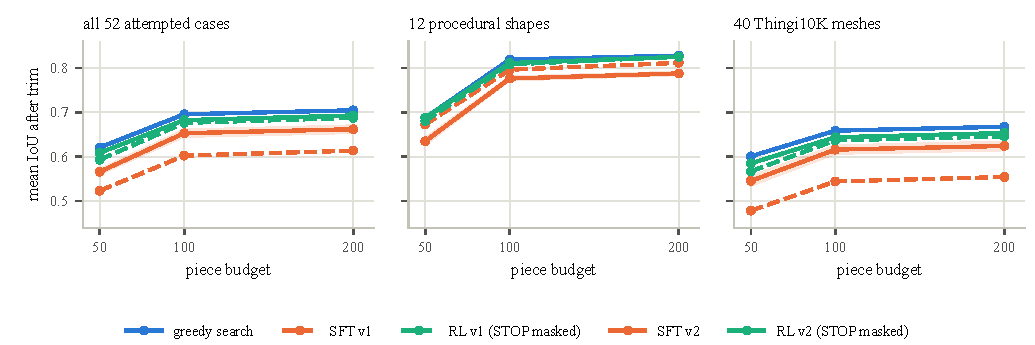
\includegraphics[width=\linewidth]{budget}
  \caption{Fidelity against piece budget for the search (blue), imitation (orange) and reinforcement learning
  (green) on the v1 data (dashed) and the v2 data (solid). Bands are the range over two training seeds. Every arm
  gains most between 50 and 100 pieces and little between 100 and 200, because the cap rarely binds: the mean build
  has about 39 pieces at the 200 cap.}
  \label{fig:budget}
\end{figure}

\subsection{Piece budget versus fidelity}
Fidelity is a concave function of the budget for every generator (Figure~\ref{fig:budget}). From 50 to 100 pieces the
search gains 0.075 and the best learned arm 0.074; from 100 to 200 they gain 0.009 and 0.012. The reason is visible in
the records: at the 200 cap the mean build has about 39 pieces and the cap is the stopping reason for almost no
case. Both the search and the policy stop when no supported, non-overlapping placement that covers a target cell
remains, which for these shapes happens long before 200 bricks. Fifty pieces, by contrast, truncates most real
meshes mid-build. The practical reading for a designer is that on this grid a 100-piece budget buys nearly all the
fidelity that 200 does. The ordering of the arms is the same at every budget, so the comparison below is reported at
200 without loss.

\subsection{Learned policy versus hand-written search}
\begin{figure}[t]
  \centering
  \begin{minipage}[t]{0.48\linewidth}
    \centering
    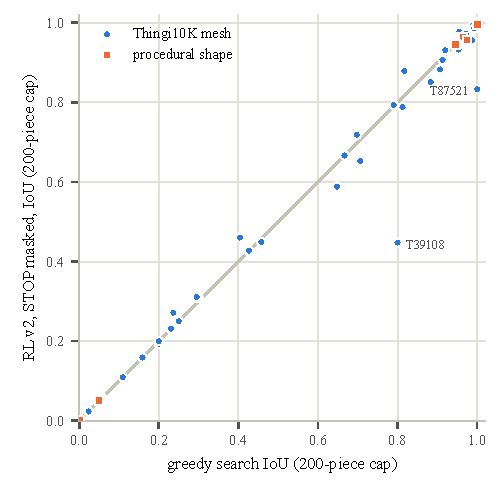
\includegraphics[width=\linewidth]{scatter}
    \caption{Per-case fidelity at the 200-piece cap, RL v2 with STOP masked against the greedy search. Most cases
    lie on the diagonal; the head-to-head record (wins / losses / ties) is \hhRlVTwoNostopVsGreedyVOne. The honeycomb
    pot T39108 is the one large loss.}
    \label{fig:scatter}
  \end{minipage}\hfill
  \begin{minipage}[t]{0.48\linewidth}
    \centering
    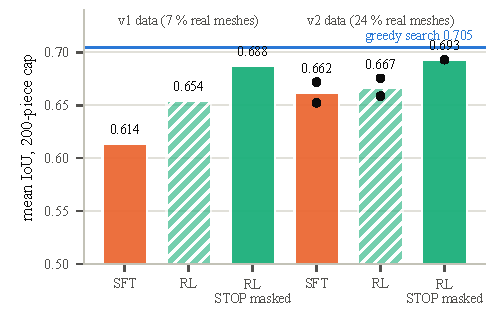
\includegraphics[width=\linewidth]{ladder}
    \caption{The ladder at the 200-piece cap. Hatched bars use the learned STOP; dots are the two training seeds of
    the v2 arms. Rebalancing the data moved SFT up, RL added more, and masking STOP added the rest.}
    \label{fig:ladder}
  \end{minipage}
\end{figure}

The RL v2 policy with STOP masked is within 0.012 mean IoU of the search at every budget. On the 12 procedural shapes
it ties (\meanRlVTwoNostopProc{} vs \meanGreedyVOneProc); on the 40 real meshes it trails by 0.015 (\meanRlVTwoNostopReal{} vs
\meanGreedyVOneReal). Its validity count (\validRlVTwoNostop/53) and model-stability count (\stableRlVTwoNostop/53) equal the
search's; the two invalid cases are the adversarial fixtures that no generator can build, so 51 is the ceiling. It
decodes in \secsRlVTwoNostop\,s per case against the search's \secsGreedyVOne\,s. Figure~\ref{fig:scatter} shows the per-case
picture: the median case is a tie, the head-to-head record is \hhRlVTwoNostopVsGreedyVOne{} (wins / losses / ties), and the
remaining gap sits in a handful of real meshes, one of which (a honeycomb pot, Section~\ref{sec:failures}) accounts for most of it.

Two comparisons bound what this means. Against its own SFT initialisation the RL policy's record is
\hhRlVTwoNostopVsSftVTwo{} (seed 0) and \hhRlVTwoSOneNostopVsSftVTwoSOne{} (seed 1). Against a test-time-compute baseline, best-of-8 sampling
from the v1 SFT policy at about seven times the decode cost, the single-sample RL v1 policy with STOP masked scores
\meanRlVOneNostopTwoHundred{} against 0.686: RL's advantage over sampling is cost, not ceiling.

\subsection{What produced the gain: data, RL, decode rule}
\label{sec:ladder}
Figure~\ref{fig:ladder} separates the three changes between the first learned arm and the last.
\begin{itemize}
  \item \textbf{Data.} The same SFT recipe on the v2 pool, which has four times as many real meshes and draws half of
  each batch from them, moves SFT from \meanSftVOneTwoHundred{} to \famSftVTwoTwoHundred{} (mean of two seeds, range
  \famloSftVTwoTwoHundred--\famhiSftVTwoTwoHundred). Given the 0.02 spread between seeds at the SFT stage, we state this gain as +0.04 to +0.06.
  \item \textbf{RL.} On the v1 data RL adds +0.040 over SFT with the learned stop (\meanSftVOneTwoHundred{} $\to$ \meanRlVOneTwoHundred).
  On the v2 data, with STOP masked, RL adds +0.021 to seed 0 and +0.041 to seed 1, and both seeds land on
  \famRlVTwoNostopTwoHundred. RL beats its own initialisation 26 to 3 and 27 to 9 head to head. Where the gain comes from is
  shown by the diagnostic fields: on the v1 ladder, fragmented builds fall from 27 to 22 of 52 and the mean number of
  pieces removed by the trim falls from 6.0 to 3.2. Figure~\ref{fig:curves} shows the training curves: validation IoU
  rises from the SFT value to within 0.02 of the teacher on the same subset, fragmentation roughly halves, and policy
  entropy stays near 1.3 to 1.6 nats with the KL to the initial policy around 0.2 to 0.3, so the policy moved without
  collapsing.
  \item \textbf{Decode rule.} Masking the learned stop adds +0.034 to RL v1 and +0.034 (seed 0) / +0.018 (seed 1) to
  RL v2. One caveat belongs here: with its \emph{own} stop, RL v2 (\meanRlVTwoTwoHundred) is below SFT v2
  (\meanSftVTwoTwoHundred) on the mean, because the RL policy stops at zero pieces on a few real meshes; the RL gain is
  only realised once stop is masked (Section~\ref{sec:stop}).
\end{itemize}

\begin{figure}[t]
  \centering
  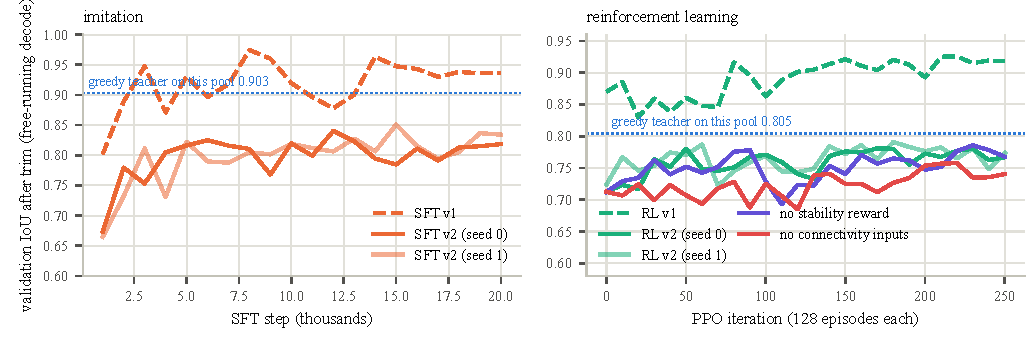
\includegraphics[width=\linewidth]{curves}
  \caption{Training curves. Left: free-running validation IoU during imitation (every 1000 steps); the v1 pool is
  almost entirely procedural and its teacher reaches 0.903 on it, the v2 pool is half real meshes and harder. Right:
  validation IoU during PPO (every 10 iterations) for both v2 seeds, the v1 run and the two ablations; the dotted
  lines are the greedy teacher on the same validation subsets.}
  \label{fig:curves}
\end{figure}

\subsection{Two training seeds}
\label{sec:seeds}
Every arm of the v2 ladder was retrained end to end with a second seed (Table~\ref{tab:seeds}). The headline reproduces:
RL v2 with STOP masked scores \famloRlVTwoNostopTwoHundred{} and \famhiRlVTwoNostopTwoHundred{} at the 200 cap, 0.012 behind the search either
way, and wins 10 and 11 cases against it. The per-case picture is also stable: the same 12 cases are lost to the search
in both seeds and the same 6 real meshes are won in both. The one count where seed 1 is worse is stability, 47
against 49 stable builds at the 200 cap (validity is identical at 51). The SFT stage, by contrast, differs by 0.020
between seeds; RL removes that spread. Two seeds give a range, not a confidence interval, and we report both numbers
rather than a mean with an error bar.

\begin{table}[t]
  \centering\small
  \caption{The v2 ladder for both training seeds at the 200-piece cap (mean IoU over attempted cases; wins / losses /
  ties against the search). The v1 arms and the ablations are single-seed.}
  \label{tab:seeds}
  \footnotesize\setlength{\tabcolsep}{3pt}
  \begin{tabular}{lccccccc}
    \toprule
    arm & s0 & s1 & procedural s0 / s1 & Thingi10K s0 / s1 & valid & stable & vs search s0; s1 \\
    \midrule
    SFT v2 & \meanSftVTwoTwoHundred & \meanSftVTwoSOneTwoHundred & \meanSftVTwoProc{} / \meanSftVTwoSOneProc & \meanSftVTwoReal{} / \meanSftVTwoSOneReal & \validSftVTwo{} / \validSftVTwoSOne & \stableSftVTwo{} / \stableSftVTwoSOne & \hhSftVTwoVsGreedyVOne; 4 / 28 / 20 \\
    RL v2 (learned STOP) & \meanRlVTwoTwoHundred & \meanRlVTwoSOneTwoHundred & \meanRlVTwoProc{} / \meanRlVTwoSOneProc & \meanRlVTwoReal{} / \meanRlVTwoSOneReal & \validRlVTwo{} / \validRlVTwoSOne & \stableRlVTwo{} / \stableRlVTwoSOne & 7 / 27 / 18; 7 / 25 / 20 \\
    RL v2, STOP masked & \meanRlVTwoNostopTwoHundred & \meanRlVTwoSOneNostopTwoHundred & \meanRlVTwoNostopProc{} / \meanRlVTwoSOneNostopProc & \meanRlVTwoNostopReal{} / \meanRlVTwoSOneNostopReal & \validRlVTwoNostop{} / \validRlVTwoSOneNostop & \stableRlVTwoNostop{} / \stableRlVTwoSOneNostop & \hhRlVTwoNostopVsGreedyVOne; \hhRlVTwoSOneNostopVsGreedyVOne \\
    \bottomrule
  \end{tabular}
\end{table}

\subsection{The stop action}
\label{sec:stop}
Table~\ref{tab:stop} (Appendix~\ref{app:stop}) is the decision table, computed on the SFT test split before each
checkpoint touched the benchmark. Masking the stop action never costs anything on procedural shapes and gains 0.03 to 0.09 on real meshes for
all five RL checkpoints (two seeds, two ablations, and v1), so the masked decode is the one reported for each. On the
benchmark the learned stop is the cause of every zero-piece build: the policy stops before placing anything on three
to six real meshes per checkpoint, different meshes for different seeds (seed 0: four meshes; seed 1: three; only one
in common). Figure~\ref{fig:stops} shows how builds end. Our reading is that the policy learned that on shapes where
every remaining candidate looks poor, stopping has the highest expected value under its own future behaviour, even
though the terminal reward penalises exactly that and half the RL episodes were real meshes. Masked decoding forces
the policy to keep tiling and lets the trim keep the largest connected part; it fragments more often (25 of 40 real
builds have pieces removed by the trim, against 14 with the learned stop) but ends with more of the target covered.


\begin{figure}[t]
  \centering
  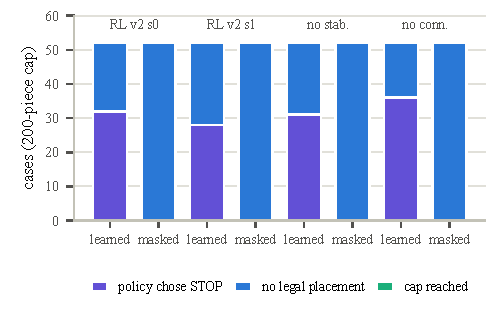
\includegraphics[width=0.6\linewidth]{stops}
  \caption{Why builds end at the 200-piece cap, for each RL checkpoint with the learned and the masked stop. The cap
  itself is never reached. With the learned stop, the policy chooses to stop on 28 to 36 of 52 cases, including a
  few at zero pieces.}
  \label{fig:stops}
\end{figure}

\subsection{Ablations}
\label{sec:ablations}
Two arms were retrained from the same seed-0 SFT checkpoint with the RL v2 settings, changing one thing each
(Table~\ref{tab:ablations}).

\begin{table}[t]
  \centering\small
  \caption{Ablations of RL v2 at the 200-piece cap (single seed; STOP masked unless stated). Wins / losses / ties are
  against the full RL v2 with STOP masked. Stable means \stablenote.}
  \label{tab:ablations}
  \begin{tabular}{lcccccc}
    \toprule
    arm & mean IoU & procedural & Thingi10K & valid & stable & vs RL v2 \\
    \midrule
    RL v2, STOP masked (reference) & \meanRlVTwoNostopTwoHundred & \meanRlVTwoNostopProc & \meanRlVTwoNostopReal & \validRlVTwoNostop & \stableRlVTwoNostop & -- \\
    no stability reward & \meanRlVTwoNostabNostopTwoHundred & \meanRlVTwoNostabNostopProc & \meanRlVTwoNostabNostopReal & \validRlVTwoNostabNostop & \stableRlVTwoNostabNostop & \hhRlVTwoNostabNostopVsRlVTwoNostop \\
    no connectivity inputs & \meanRlVTwoNoconnNostopTwoHundred & \meanRlVTwoNoconnNostopProc & \meanRlVTwoNoconnNostopReal & \validRlVTwoNoconnNostop & \stableRlVTwoNoconnNostop & \hhRlVTwoNoconnNostopVsRlVTwoNostop \\
    \midrule
    no stability reward, learned STOP & \meanRlVTwoNostabTwoHundred & \meanRlVTwoNostabProc & \meanRlVTwoNostabReal & \validRlVTwoNostab & \stableRlVTwoNostab & \\
    no connectivity inputs, learned STOP & \meanRlVTwoNoconnTwoHundred & \meanRlVTwoNoconnProc & \meanRlVTwoNoconnReal & \validRlVTwoNoconn & \stableRlVTwoNoconn & \\
    \bottomrule
  \end{tabular}
\end{table}

\paragraph{The stability reward is redundant.} With the stability term removed from the reward, the builds are
exactly as stable as with it: 147 of 153 valid builds across the three budgets, the same two real meshes unstable at
the 200 cap, identical to the search. The legality rule that every brick must rest on something, together with the
trim to one grounded component, already produces structures the force model accepts; the bonus had nothing left to
reward. Fidelity moves by 0.007 (\hhRlVTwoNostabNostopVsRlVTwoNostop{} head to head), a single-seed difference smaller than the
0.02 seed spread at the SFT stage, though one case moves a lot (the honeycomb pot falls from 0.45 to 0.25). The
clean statement is that in this setting stability comes from the hard constraints, not from reward shaping.

\paragraph{The connectivity inputs matter where the policy judges on its own.} Removing the main-component channel and
the two connectivity features costs 0.064 on the benchmark under the learned stop (\meanRlVTwoNoconnTwoHundred{} vs
\meanRlVTwoTwoHundred), with six real meshes ending at zero pieces; it costs 0.035 on the 260-example test split with stop masked
(Table~\ref{tab:stop} in Appendix~\ref{app:stop}, 0.805 vs 0.840) and 0.023 on the validation curve. Yet on the 52-case benchmark with stop
masked the means are within 0.003 (\meanRlVTwoNoconnNostopTwoHundred{} vs \meanRlVTwoNostopTwoHundred), because one large win on the honeycomb
pot (0.78 vs 0.45) offsets 18 losses to 7 wins. Head to head it is the weaker policy; the benchmark mean is too
coarse to show it. The features' main job is telling the policy which candidates attach to the main component and
when a build is finished. With stop masked, the trim does that cleanup after decoding for free.

\subsection{Failure analysis}
\label{sec:failures}
\begin{figure}[p]
  \centering
  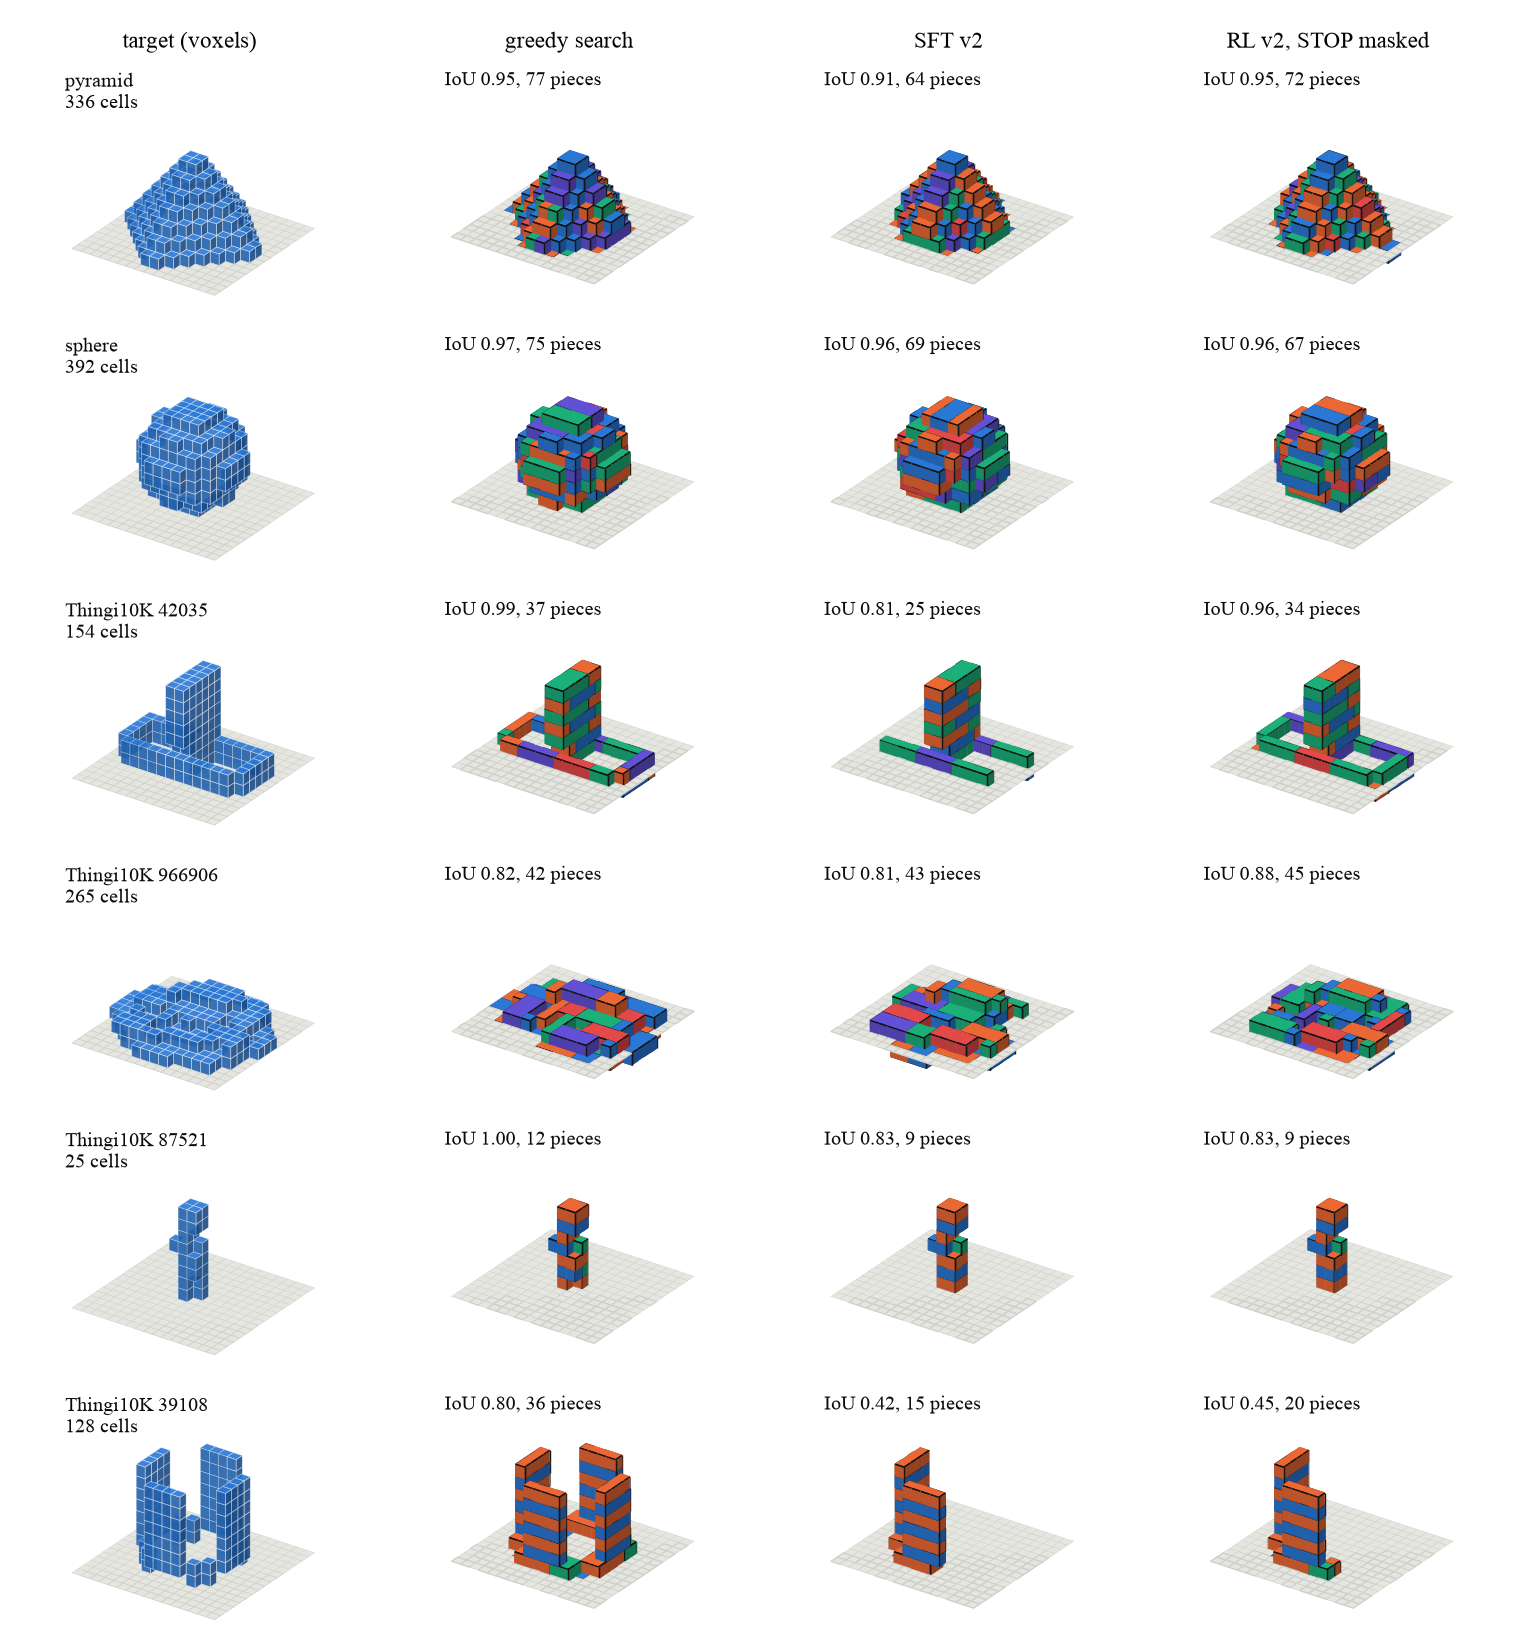
\includegraphics[width=\linewidth]{gallery}
  \caption{Six benchmark cases at the 200-piece cap: the voxel target, the search, SFT v2 and RL v2 with STOP masked.
  Rows: two procedural shapes (the pyramid shows SFT dropping pieces that RL recovers), a mesh where RL recovers most
  of SFT's loss (T42035), the largest RL win (T966906), a small mesh lost by both learned arms (T87521), and the
  honeycomb pot (T39108), the one case any learned generator loses by more than 0.35. Colours separate neighbouring
  bricks and carry no meaning.}
  \label{fig:gallery}
\end{figure}

Figure~\ref{fig:gallery} shows where the remaining gap lives. Twelve cases are lost to the search in both seeds: two
procedural shapes by at most 0.02 (sphere, wedge) and ten real meshes. One shape class dominates: thin-walled shells
with interior structure. The honeycomb pot (T39108) is the only case any learned generator loses by more than 0.35
(search 0.80, RL 0.45 and 0.42 across seeds): the policy tiles the outer walls as it would a solid and 19 of its 39
pieces are removed by the trim as unconnected. The search's exhaustive scan of every placement at every step, with
hard cells first, still beats a learned preference on such shapes. The six real meshes won in both seeds are the
opposite: broad, low shapes where the policy's placements interlock better than the search's layer-wise tiling and
the trim removes less. Finally, the two cases that are valid but unstable under the model for every generator are
tiny fragments (3 to 5 pieces with overhangs) left after trimming a mesh that occupies fewer than 90 of the 2048
cells; grid resolution, not the generator, is the limit there.
